\chapter{Análisis de Resultados}
\section{Capturas del programa en ejecución}

A continuación se presenta en orden el proceso de ejecución del programa, donde primeramente se muestra el código en ejecución con un ejemplo chico.\newline
\newpage

\begin{enumerate}
\item Iniciamos el programa, donde nos pide que introduzcamos una cadena o de lo contrario al presionar enter se generara una aleatoria, para nuestro ejemplo digitamos 0000011111 que vienen siendo 5 ceros y 5 unos. Observar la Figura 2.1.

\begin{figure}[h]
\begin{minipage}{0.3\textwidth}
    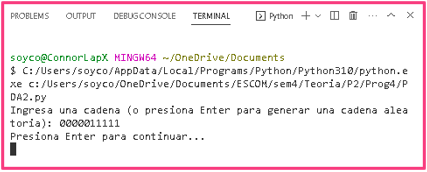
\includegraphics[width=4\linewidth]{Images/Cap1.png}
\end{minipage}
\caption{Inicio del programa en terminal.}
\label{fig:imagen}
\end{figure}
\newpage
\item Aquí se puede visualizar la animación del autómata pila. Se inserta X. Observar la Figura 2.2.\newline
\begin{figure}[h]
\begin{minipage}{0.3\textwidth}
    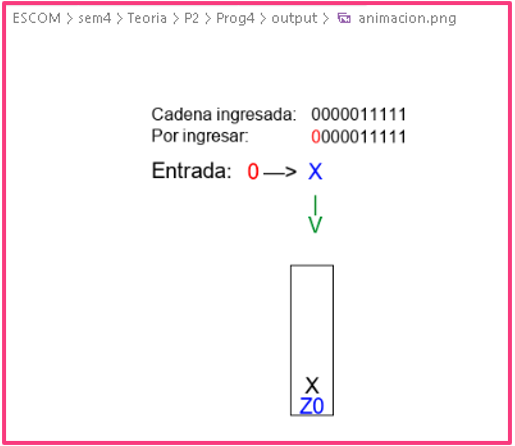
\includegraphics[width=3.5\linewidth]{Images/Cap2.png}
\end{minipage}
\caption{Animación primera parte.}
\label{fig:imagen}
\end{figure}

\newpage
\item Segunda parte de animación y terminal, se inserta X. Observar la Figura 2.3.
\begin{figure}[h]
%\begin{minipage}{0.3\textwidth}
    \begin{center}
    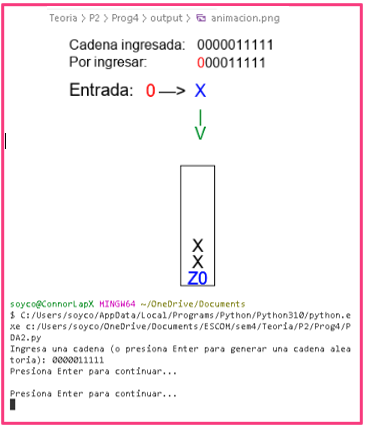
\includegraphics[width=0.7\linewidth]{Images/Cap3.png}
    \end{center}
%\end{minipage}
\caption{Segunda parte de animación y terminal.}
\label{fig:imagen}
\end{figure}

\newpage
\item Tercera parte de animación y terminal, se inserta X. Observar la Figura 2.4.
\begin{figure}[h]
%\begin{minipage}{0.3\textwidth}
    \begin{center}
    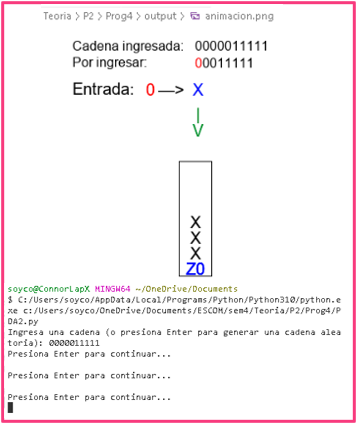
\includegraphics[width=0.7\linewidth]{Images/Cap4.png}
    \end{center}
%\end{minipage}
\caption{Tercera parte de animación y terminal.}
\label{fig:imagen}
\end{figure}

\newpage
\item Cuarta parte de animación y terminal, se inserta X. Observar la figura 2.5.

\begin{figure}[h]
%\begin{minipage}{0.3\textwidth}
    \begin{center}
    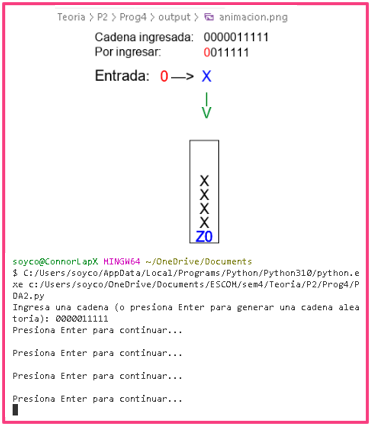
\includegraphics[width=0.7\linewidth]{Images/Cap5.png}
    \end{center}
%\end{minipage}
\caption{Cuarta parte de animación y terminal.}
\label{fig:imagen}
\end{figure}

\newpage
\item Quinta parte de animación y terminal, se inserta X. Observar la figura 2.6.

\begin{figure}[h]
%\begin{minipage}{0.3\textwidth}
    \begin{center}
    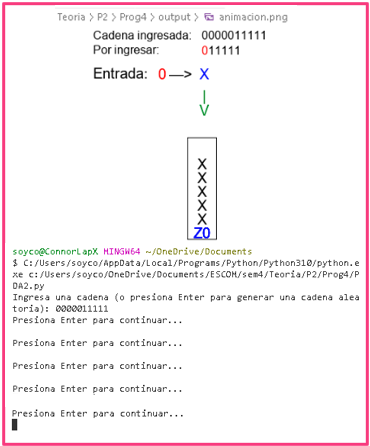
\includegraphics[width=0.7\linewidth]{Images/Cap6.png}
    \end{center}
%\end{minipage}
\caption{Quinta parte de animación y terminal.}
\label{fig:imagen}
\end{figure}
\newpage
\item Sexta parte de animación y terminal, se elimina X. Observar la figura 2.7.

\begin{figure}[h]
%\begin{minipage}{0.3\textwidth}
    \begin{center}
    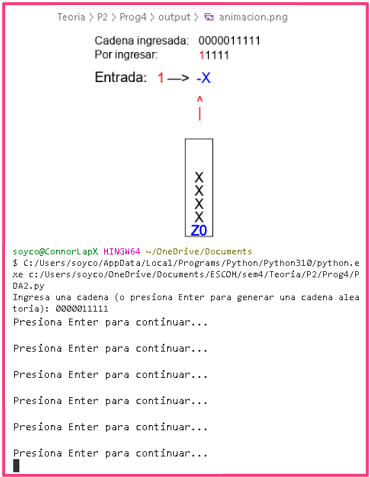
\includegraphics[width=0.7\linewidth]{Images/Cap7.png}
    \end{center}
%\end{minipage}
\caption{Sexta parte de animación y terminal.}
\label{fig:imagen}
\end{figure}
\newpage
\item Séptima parte de animación y terminal, se elimina X. Observar figura 2.8.

\begin{figure}[h]
%\begin{minipage}{0.3\textwidth}
    \begin{center}
    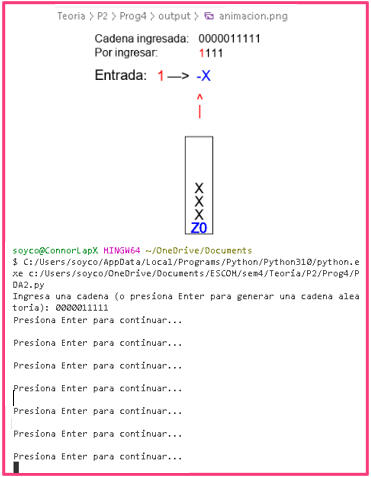
\includegraphics[width=0.6\linewidth]{Images/Cap8.png}
    \end{center}
%\end{minipage}
\caption{Séptima parte de animación y terminal.}
\label{fig:imagen}
\end{figure}

\newpage
\item Octava parte de animación y terminal, se elimina X. Observar figura 2.9.

\begin{figure}[h]
%\begin{minipage}{0.3\textwidth}
    \begin{center}
    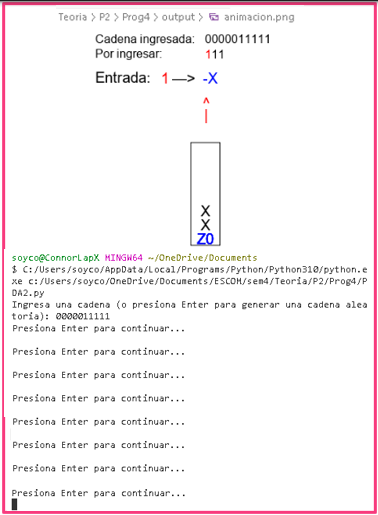
\includegraphics[width=0.6\linewidth]{Images/Cap9.png}
    \end{center}
%\end{minipage}
\caption{Octava parte de animación y terminal.}
\label{fig:imagen}
\end{figure}

\newpage
\item Novena parte de animación y terminal, se elimina X. Observar figura 2.10.

\begin{figure}[h]
%\begin{minipage}{0.3\textwidth}
    \begin{center}
    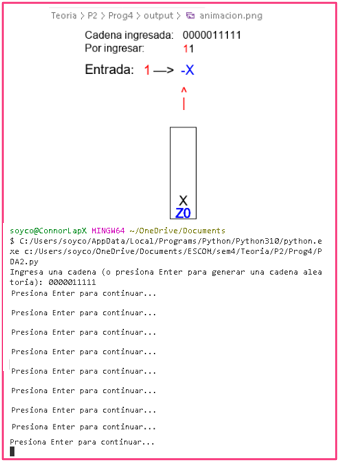
\includegraphics[width=0.6\linewidth]{Images/Cap10.png}
    \end{center}
%\end{minipage}
\caption{Novena parte de animación y terminal.}
\label{fig:imagen}
\end{figure}

\newpage
\item Décima parte de animación y terminal, se elimina X. Observar la figura 2.11.

\begin{figure}[h]
%\begin{minipage}{0.3\textwidth}
    \begin{center}
    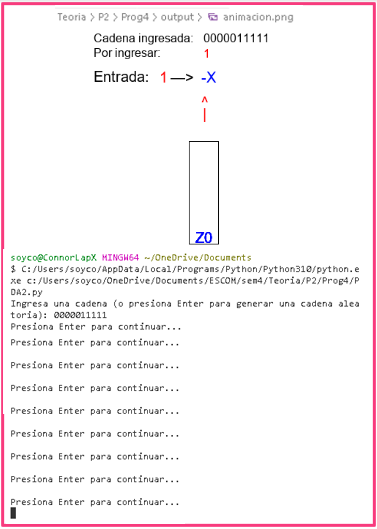
\includegraphics[width=0.6\linewidth]{Images/Cap11.png}
    \end{center}
%\end{minipage}
\caption{Décima parte de animación y terminal.}
\label{fig:imagen}
\end{figure}

\newpage
\item Onceava parte de animación y terminal, se recibe el vacío y, por lo tanto, se saca lo que haya en la pila, en este caso Z0. Observar la figura 2.12.

\begin{figure}[h]
%\begin{minipage}{0.3\textwidth}
    \begin{center}
    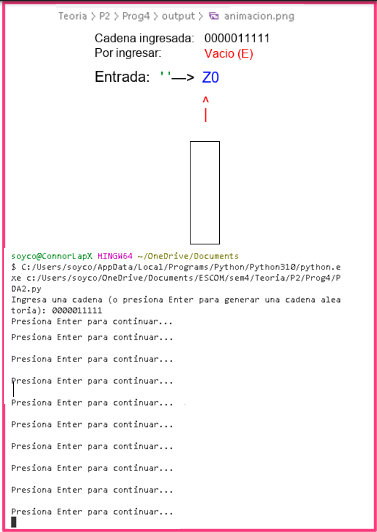
\includegraphics[width=0.6\linewidth]{Images/Cap12.png}
    \end{center}
%\end{minipage}
\caption{Onceava parte de animación y terminal.}
\label{fig:imagen}
\end{figure}

\newpage
\item Doceava parte de animación y terminal, se válida la cadena. Observar la figura 2.13.

\begin{figure}[h]
%\begin{minipage}{0.3\textwidth}
    \begin{center}
    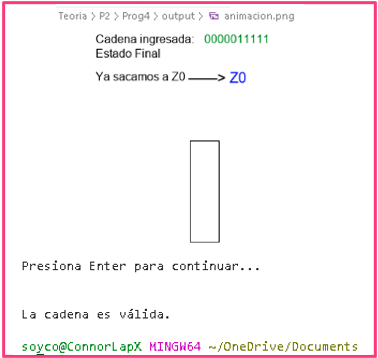
\includegraphics[width=0.6\linewidth]{Images/Cap13.png}
    \end{center}
%\end{minipage}
\caption{Doceava parte de animación y terminal.}
\label{fig:imagen}
\end{figure}
\newpage
\item Aquí podemos ver el archivo de salida de transiciones.txt, y poder visualizar como se llevó a cabo la construcción de la pila. Observar la figura 2.14.

\begin{figure}[h]
%\begin{minipage}{0.3\textwidth}
    \begin{center}
    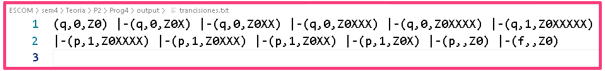
\includegraphics[width=1\linewidth]{Images/Cap14.png}
    \end{center}
%\end{minipage}
\caption{Archivo de salida de transiciones.txt.}
\label{fig:imagen}
\end{figure}
\newpage
\item En esta aparte pedimos al programa una cadena aleatoria presionando Enter, se digito aleatoriamente una cadena de tamaño 70,196. Observar la figura 2.15.

\begin{figure}[h]
%\begin{minipage}{0.3\textwidth}
    \begin{center}
    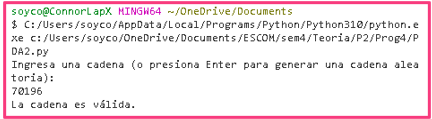
\includegraphics[width=1\linewidth]{Images/Cap15.png}
    \end{center}
%\end{minipage}
\caption{Nueva entrada aleatoria.}
\label{fig:imagen}
\end{figure}
\newpage
\item Aquí podemos ver el inicio del archivo de salida de transiciones.txt, y poder visualizar como se llevó a cabo la construcción de la pila. Observar la figura 2.16.

\begin{figure}[h]
%\begin{minipage}{0.3\textwidth}
    \begin{center}
    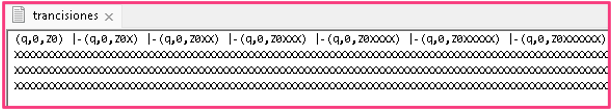
\includegraphics[width=1\linewidth]{Images/Cap16.png}
    \end{center}
%\end{minipage}
\caption{Inicio de archivo de trancisiones.txt.}
\label{fig:imagen}
\end{figure}
\newpage
\item Aquí podemos ver el final del archivo de salida de transiciones.txt, y poder visualizar como se llevó a cabo la construcción de la pila. Observar la figura 2.17.

\begin{figure}[h]
%\begin{minipage}{0.3\textwidth}
    \begin{center}
    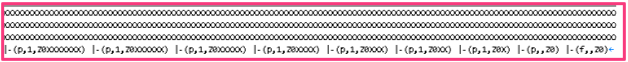
\includegraphics[width=1\linewidth]{Images/Cap17.png}
    \end{center}
%\end{minipage}
\caption{Final de archivo de trancisiones.txt .}
\label{fig:imagen}
\end{figure}
\end{enumerate}